

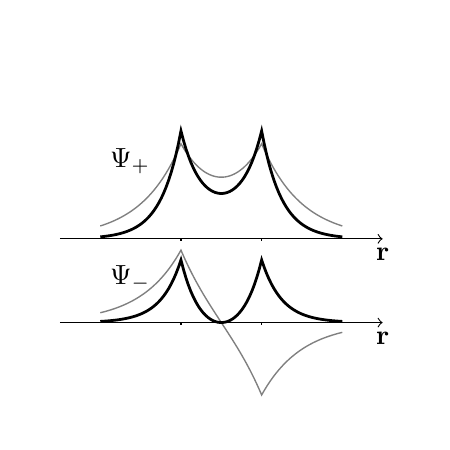
\begin{tikzpicture}
\useasboundingbox (0,0) rectangle (5,5);
%\draw (0,0) rectangle (5,5);

\begin{axis}[no markers, samples=100,
    %      ymin=-1.1, ymax=1,
         axis y line=none,
           axis x line=none,
           width= 6.5cm]
           
\addplot [domain=-3:3,  line width=0.5pt, color=gray]  
   {exp(-1 * abs(x+1)) +  exp(-1 * abs(x-1)) +1};
\addplot [domain=-3:3,  line width=0.5pt,  color=gray]  
   {exp(-1 * abs(x+1)) -  exp(-1 * abs(x-1))};

\addplot [domain=-3:3,  line width=1pt]  
   {(exp(-1 * abs(x+1)) +  exp(-1 * abs(x-1)))^2 +1};
\addplot [domain=-3:3,  line width=1pt]  
   {(exp(-1 * abs(x+1)) -  exp(-1 * abs(x-1))) ^2};


%\addplot [ domain=-3:3,  line width=1pt]   
% {exp(-1 * abs(x+1)) *  exp(-1 * abs(x-1))} ;
%

\addplot[->] coordinates   {(-4,1) (4, 1)};
\addplot[] coordinates   {(-1,1) (-1, 0.97)};
\addplot[] coordinates   {(+1,1) (+1, 0.97)};
   
\addplot[->] coordinates   {(-4,0) (4, 0)};
\addplot[] coordinates   {(-1,0) (-1, -0.03)};
\addplot[] coordinates   {(+1,0) (+1, -0.03)};
%
\node[anchor=north] at (axis cs: 4,0) {$\mathbf{r}$};
\node[anchor=north] at (axis cs: 4,1) {$\mathbf{r}$};


\node[anchor= north west] at (axis cs: -3,0.8) {$\Psi_-$};
\node[anchor= north west] at (axis cs: -3,2.2) {$\Psi_+$};
%\node[anchor= north east] at (axis cs: 1,1) {$\phi_2$};
%\node[anchor= west] at (axis cs: +1.3,-0.7) {$\frac{-1}{|\mathbf{r} - \mathbf{r}_2|}$};
%
%\node (s) [anchor= west] at (axis cs: +1.2,+0.2) {$\frac{\phi_1 \phi_2}{|\mathbf{r} - \mathbf{r}_2|}$} ;
%
%\node (k) at (axis cs: -1,+0.) {};
%
%%\draw (s) -- (k) ;
%
%%\node[anchor= south] at (axis cs: 0,0) {$\phi_1 \cdot \phi_2$};
%
%%\node[anchor=west] at (axis cs: 1,1.4) {state $e$};
%           
\end{axis}

\end{tikzpicture}

